\chapter{ADDITIONAL REORIENTATIONAL DECAY PLOTS FOR ICE-I$_\mathrm{h}$ / WATER INTERFACES}\label{dynamicAppendix}

Contained in this appendix are additional orientational decay plots of the SPC/E ice-I$_\mathrm{h}$ / water interfaces.



\begin{figure*}
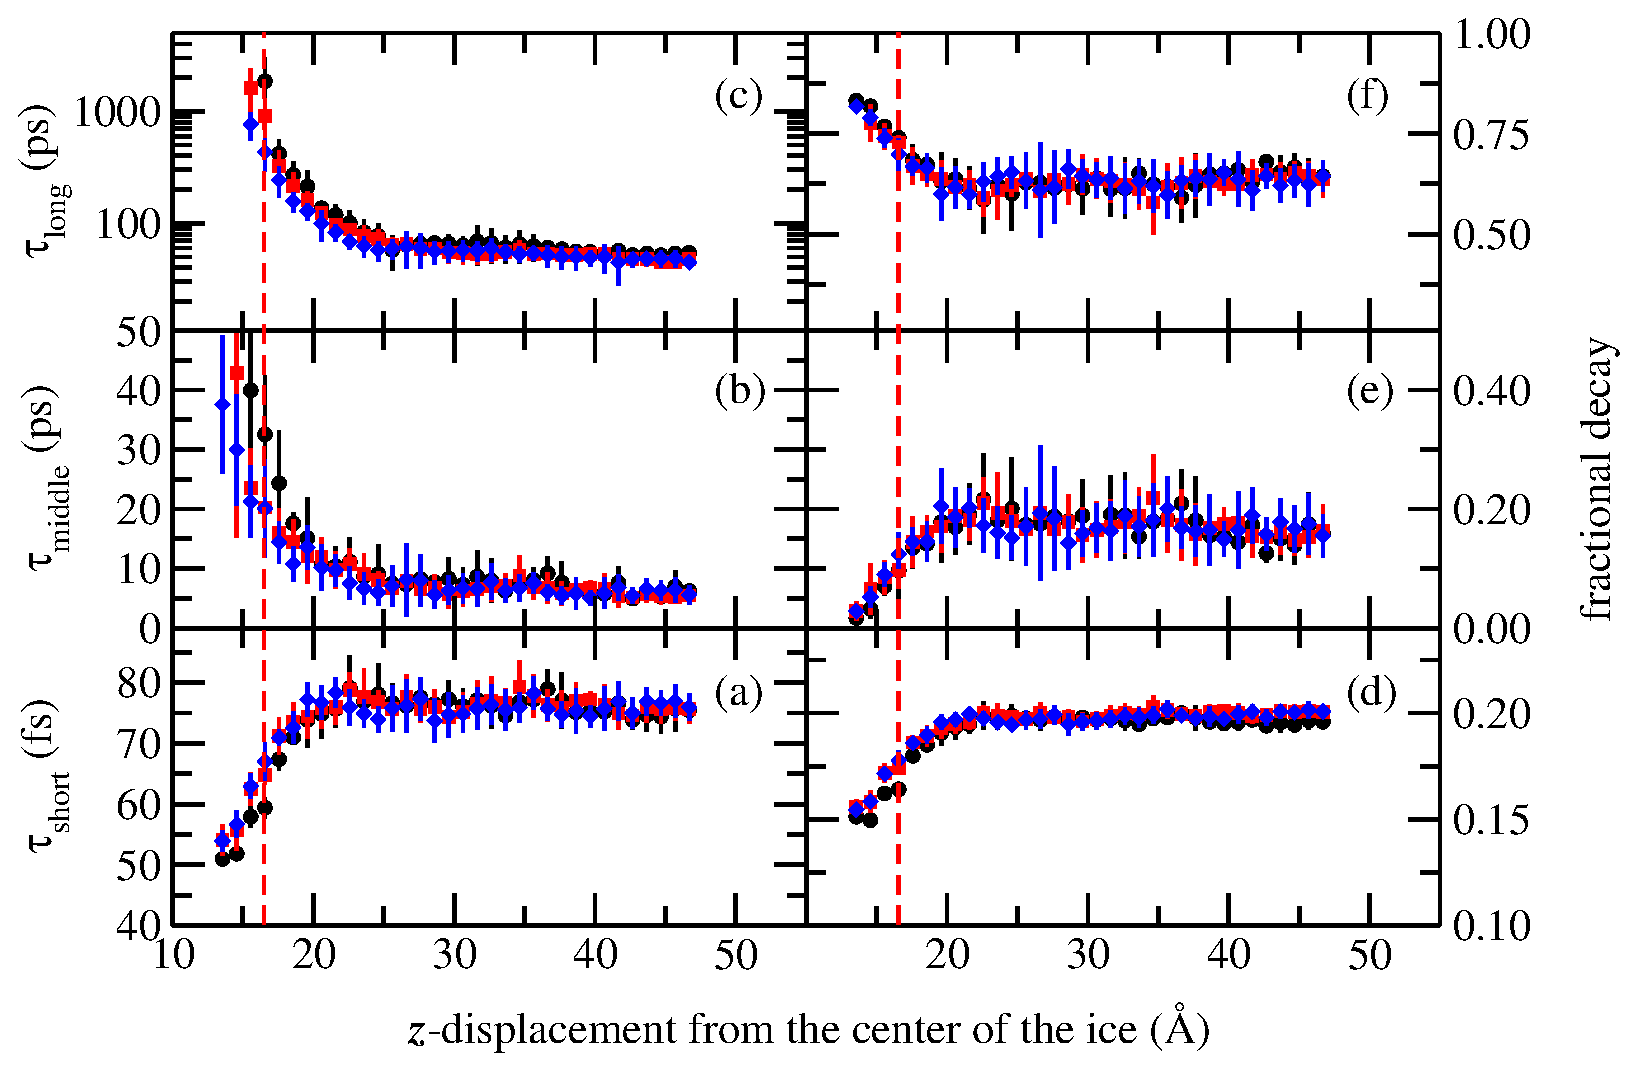
\includegraphics[width=\linewidth]{Figures/Pyr_lcorrz}
\caption{\label{fig:Pyrorient} Decay times (left) for $C_2(z,t)$ at
  the pyramidal interface, and their fractional contributions to the
  overall decay (right) fit using Equation \eqref{eq:c2}. The local
  decay constants are plotted as a function of distance from the
  center of the ice slab. The vertical dashed line indicates the Gibbs
  dividing surface determined using the local tetrahedral order
  parameter.  Results are shown for a quiescent system with no applied
  kinetic or momentum flux (black), an interface with with an imposed
  kinetic energy flux (red), and a sheared simulation (blue) with both
  kinetic and momentum fluxes.}
\end{figure*}

\begin{figure*}
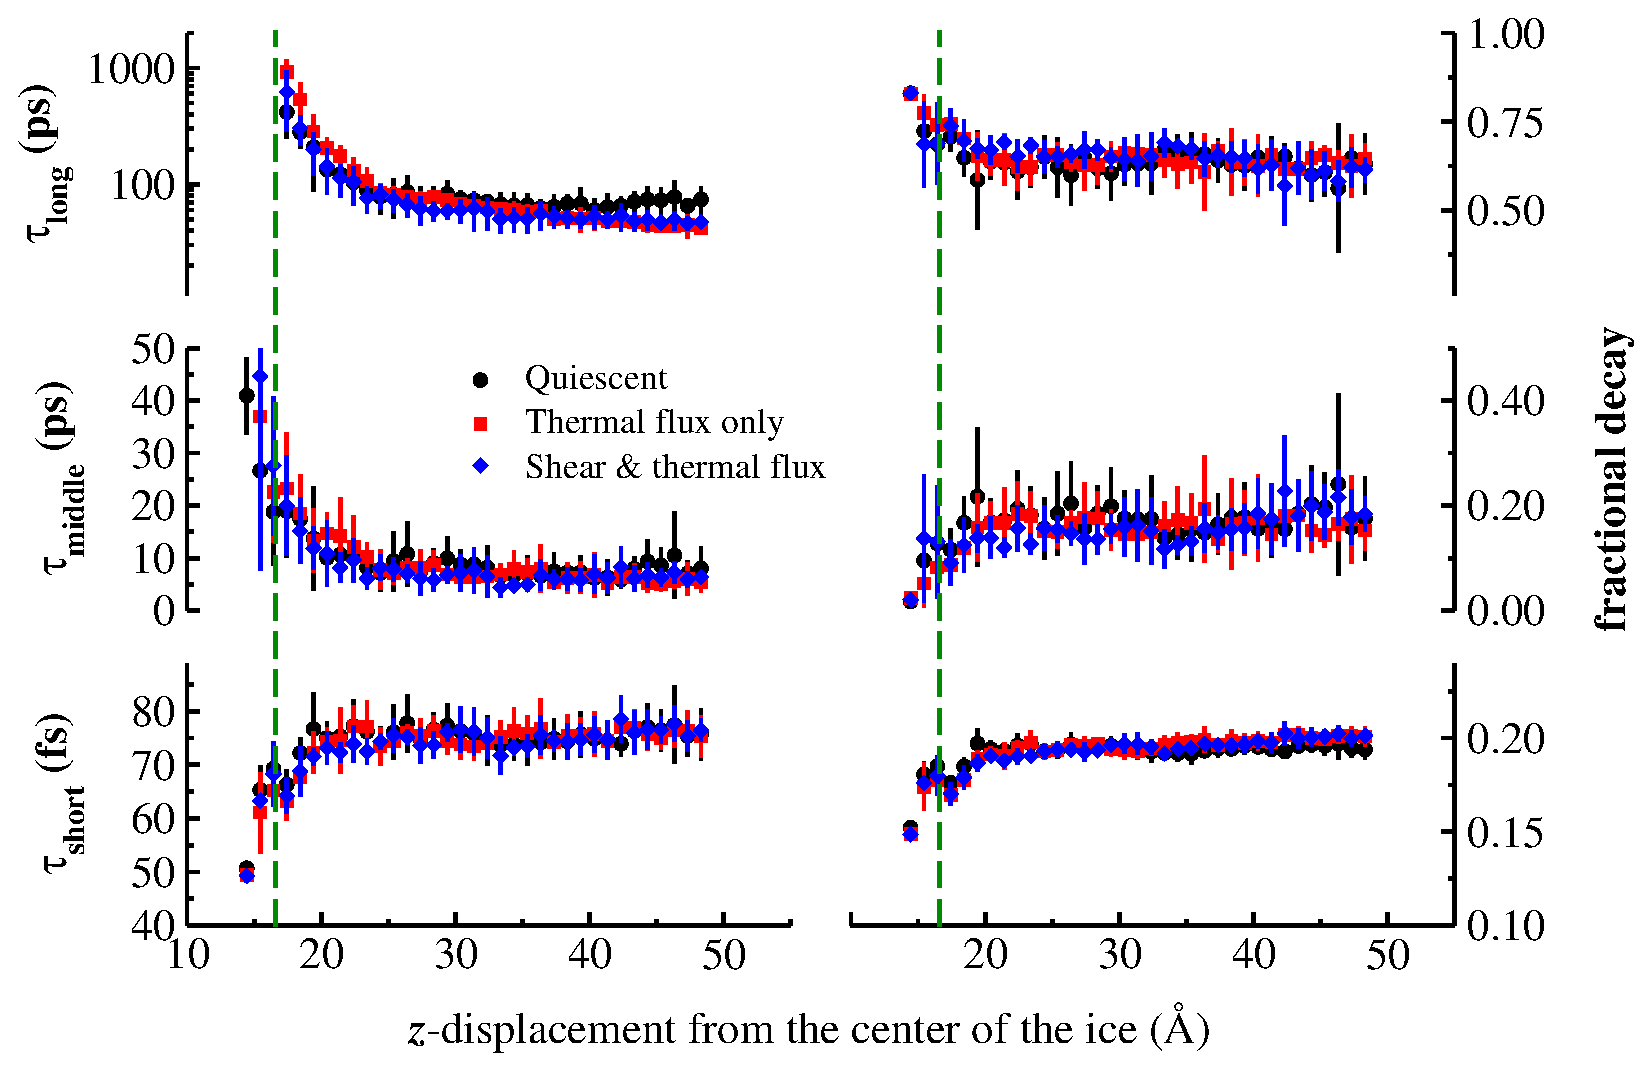
\includegraphics[width=\linewidth]{Figures/Bas_lcorrz}
\caption{\label{fig:Borient} $C_2(z,t)$ time constants for the basal
  interface.  Panel descriptions are the same as in
  Fig. \ref{fig:Pyrorient}. }
\end{figure*}

\begin{figure*}
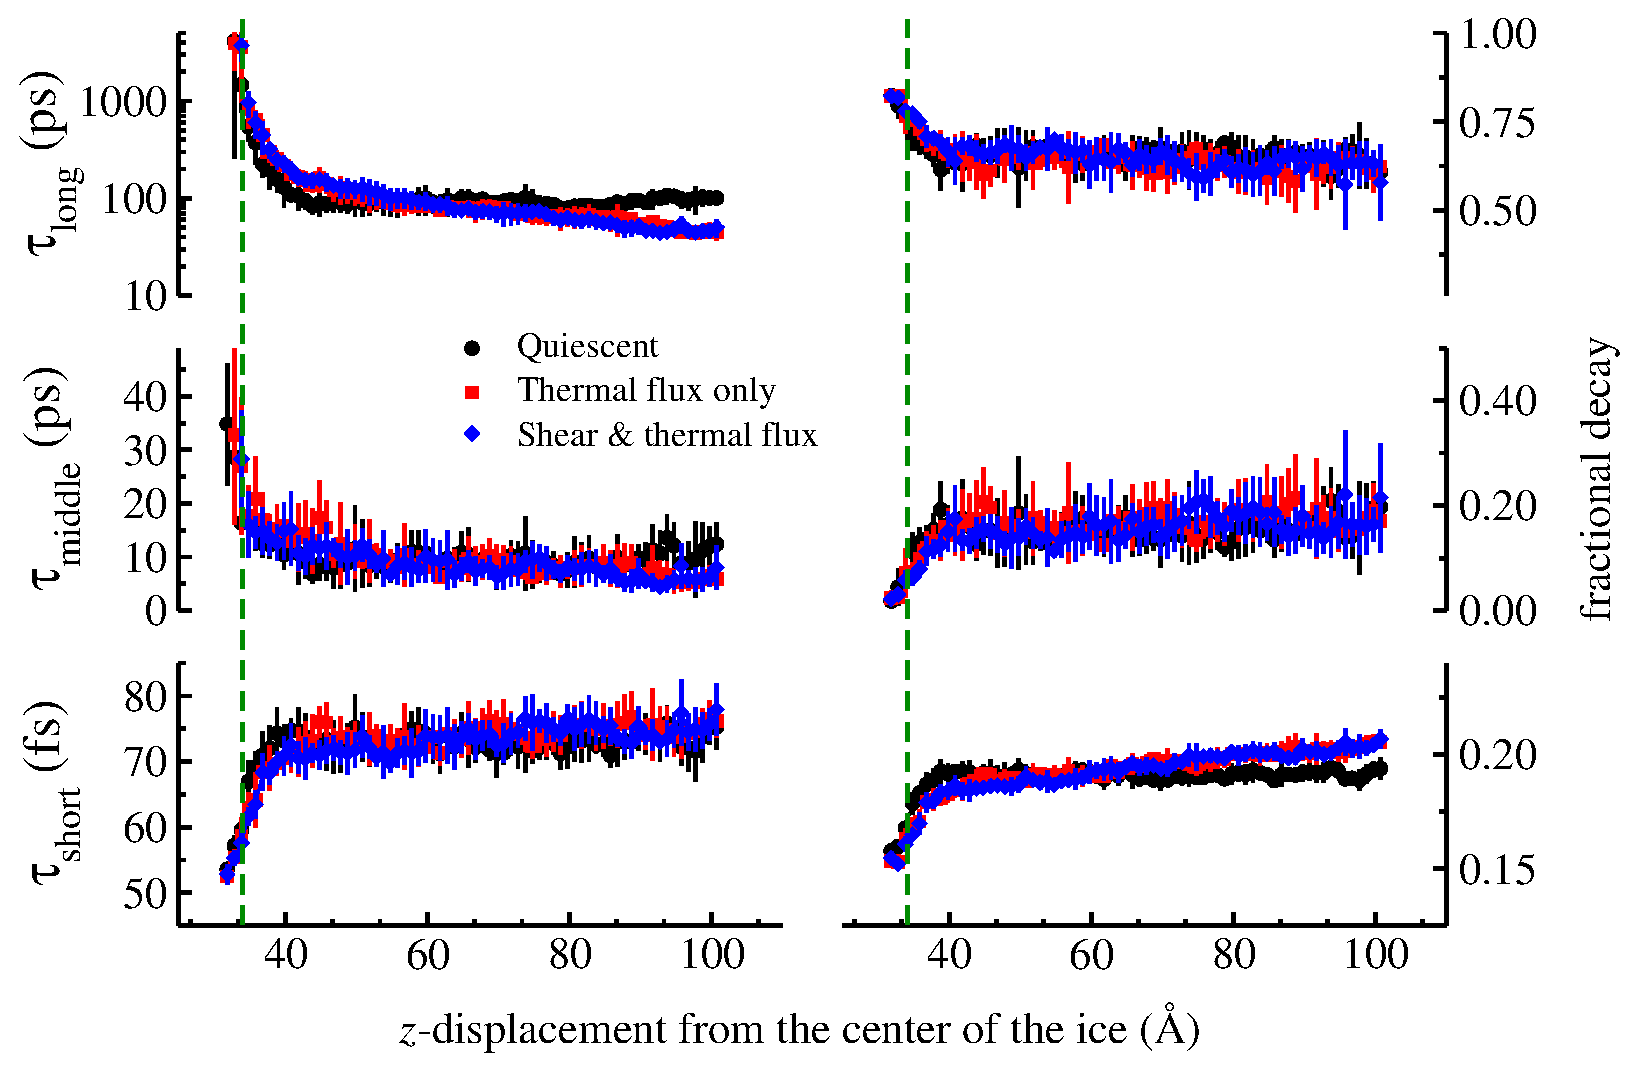
\includegraphics[width=\linewidth]{Figures/Pri_lcorrz}
\caption{\label{fig:Porient} $C_2(z,t)$ time constants for the prismatic
  interface.  Panel descriptions are the same as in
  Fig. \ref{fig:Pyrorient}.}
\end{figure*}

\begin{figure*}
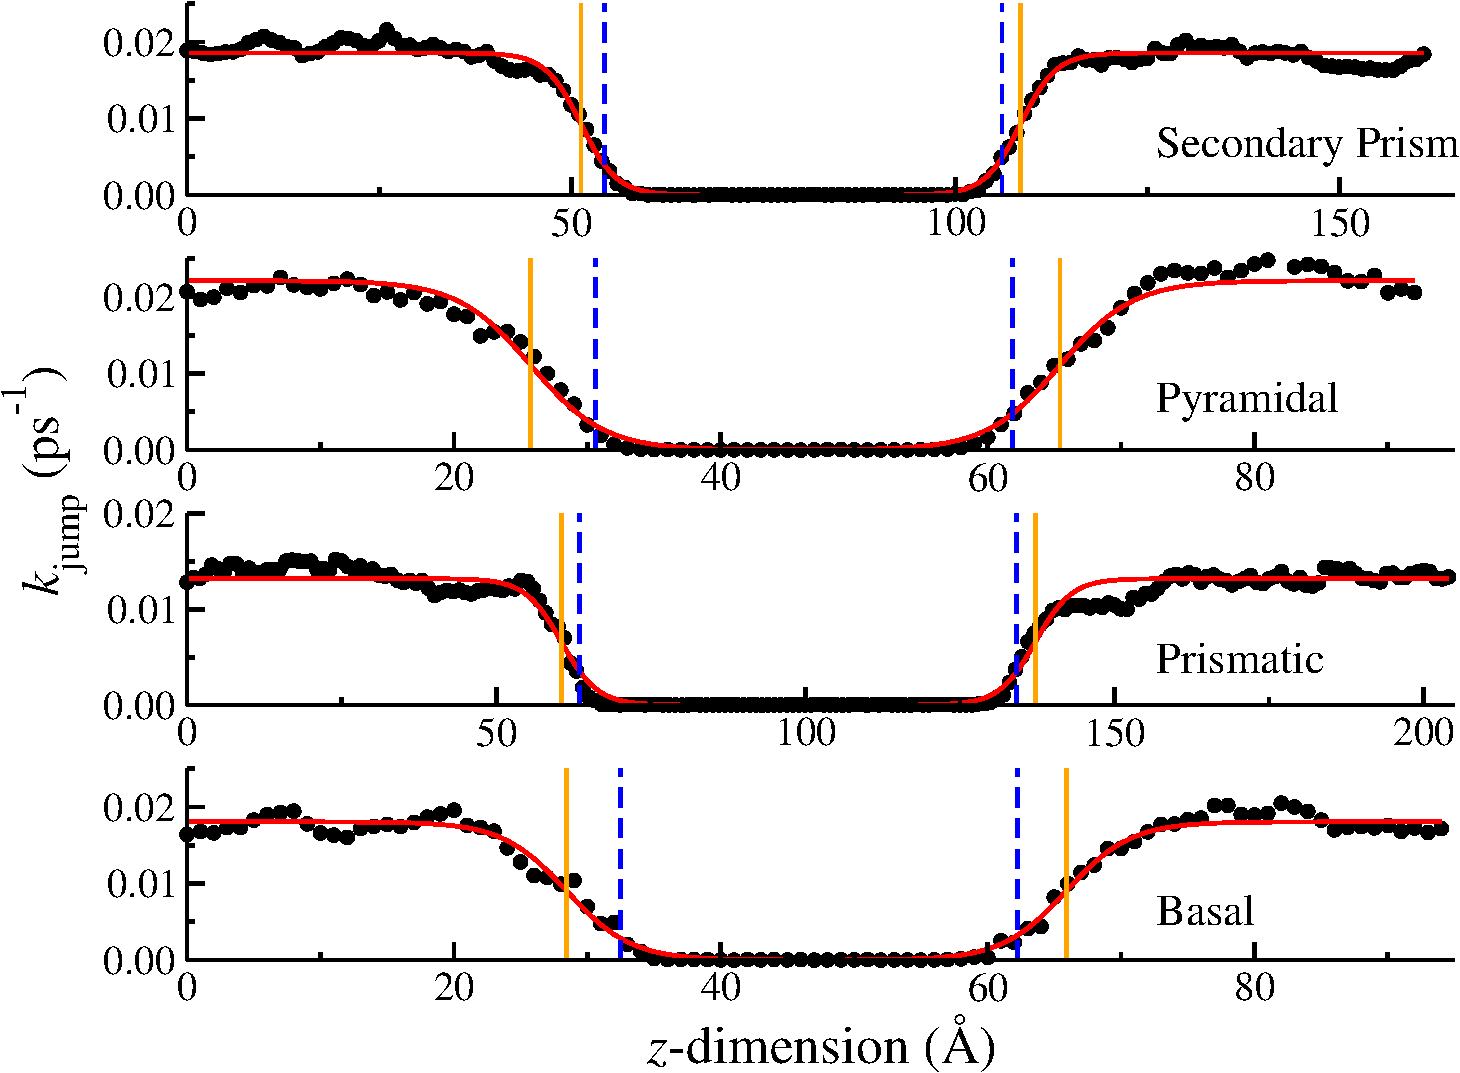
\includegraphics[width=\linewidth]{Figures/jumpRateStackedPlot2}
\caption{\label{fig:SPCEjumpRates} The jump rates,
  $k_\mathrm{jump}(z)$, for the SPC/E ice / water systems at 225 K as
  determined by Equation \eqref{tauFit}.  These are shown with a fit that
  provides a ``jump'' width, $d_\mathrm{10-90}^{jump}$. The locations
  of the structural Gibbs dividing surfaces (using tetrahedrality) are
  indicated with vertical dashed blue lines, while the locations of
  the ``jump'' interfaces are shown in orange.}
\end{figure*}


\begin{figure*}
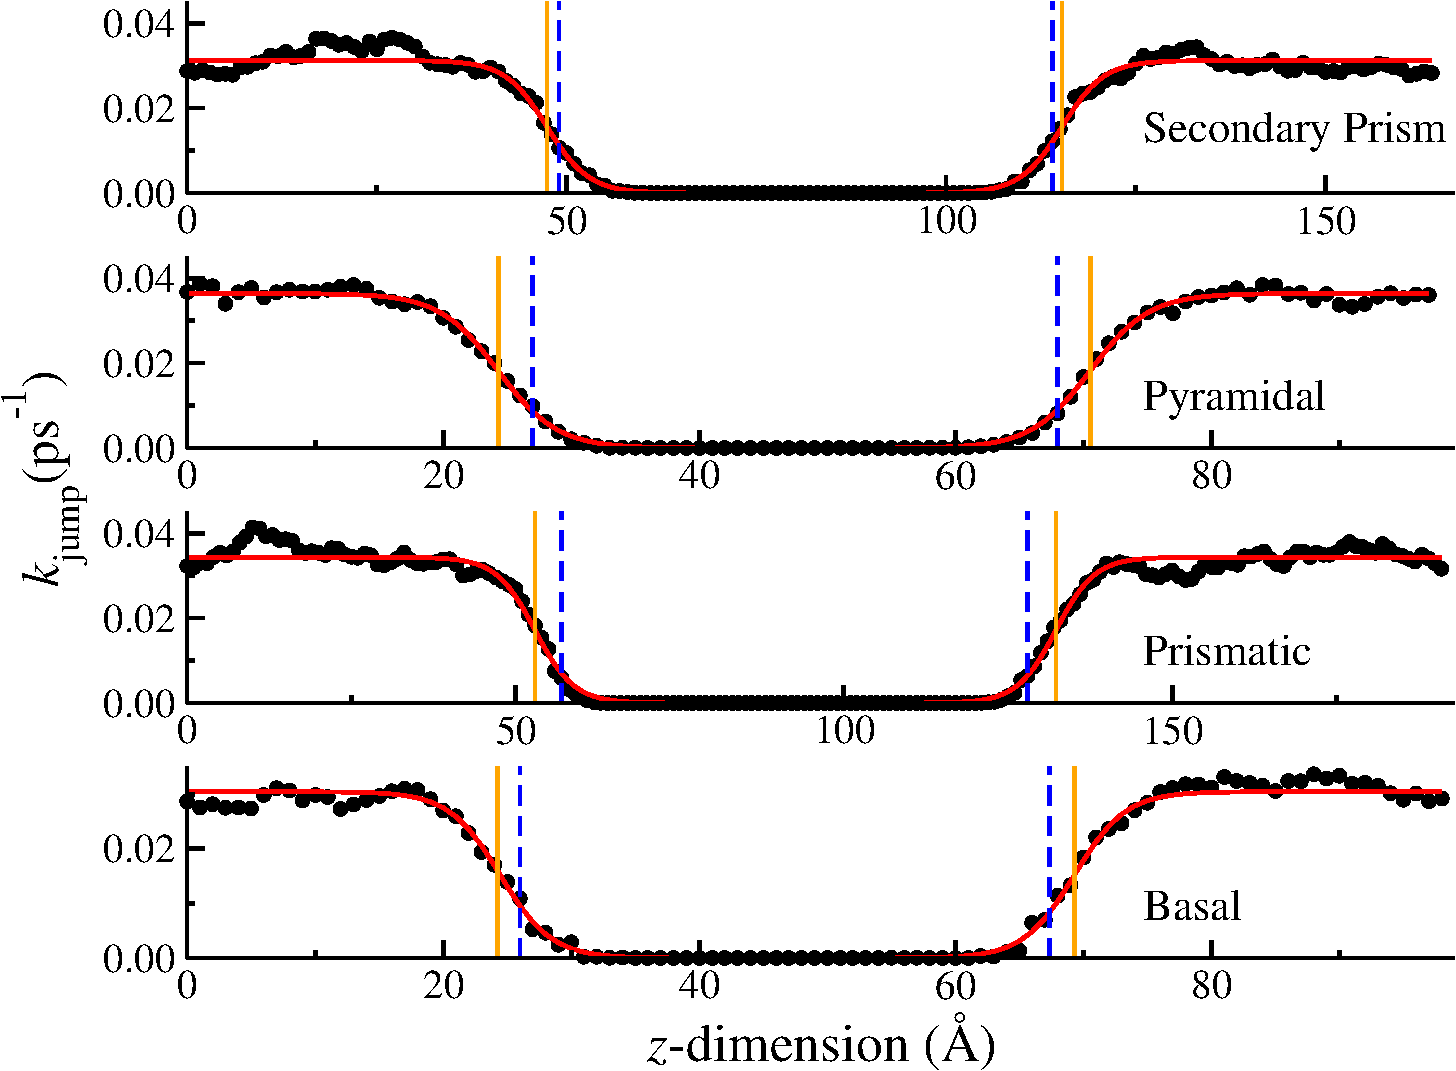
\includegraphics[width=\linewidth]{Figures/TIP4PjumpStacked}
\caption{\label{fig:TIP4PIcejumpRates} The same secondary prism hydrogen
  bond jump data as Figure \ref{fig:SPCEjumpRates}, but collected using the
  TIP4P/Ice model and at 270~K.  Note that the higher coexistence
  temperature for this model increases the observed liquid-state jump
  rates, and has brought the structural and jump interfaces much
  closer together. }
\end{figure*}